% !TeX spellcheck = en_US
\documentclass{article}
\usepackage{graphicx}
\usepackage{fancybox}
\usepackage{tikz}
\usepackage{algorithm}
\usepackage{amsmath}
\usepackage{algorithmicx}
\usepackage{algpseudocode}
\usepackage{graphicx}
\usepackage{hyperref}
\usepackage{enumitem}
\usepackage{fancybox}
\usepackage{tikz}
\usepackage{caption}
\usepackage{subcaption}

\captionsetup{labelfont={color=black,bf}}


\makeatletter
\def\BState{\State\hskip-\ALG@thistlm}
\makeatother

\algdef{SE}[DOWHILE]{Do}{doWhile}{\algorithmicdo}[1]{\algorithmicwhile\ #1}%

\title{Homework 04: Sorting}
\date{\today}
\author{Roberto Corti}

\begin{document}
	\maketitle
	\section*{Exercise 1}
	\textbf{By using the code at:}
		\begin{center}
			\url{https://github.com/albertocasagrande/AD_sorting}
		\end{center}
	\textbf{implement \texttt{INSERTION SORT}, \texttt{QUICK SORT}, \texttt{BUBBLE SORT}, \texttt{SELECTION SORT}, and \texttt{HEAP SORT}.} \\
	
	\noindent These functions are respectively implemented into the files \texttt{src/insertion\_sort.c}, \texttt{src/quick\_sort.c}, \texttt{src/bubble\_sort.c}, \texttt{src/selection\_sort.c} and  \texttt{src/heap\_sort.c}. 
	
	\section*{Exercise 2}
	\textbf{For each of the implemented algorithm, draw a curve to represent the relation between the input size and the execution-time.} \\
	
	\noindent Once implemented the sorting algorithms, in \texttt{src/main.c} I tested their performances by measuring the execution time for several input sizes $n$. We expect the following asymptotic complexities:
	\begin{itemize}
		\item \texttt{INSERTION SORT} is $O(n^2)$ (worst-case) and $\Omega(n)$ (best-case), 
		\item  \texttt{QUICK SORT} is $\Theta(n\log n)$ (average-case and best-case) and $\Theta(n^2)$ (worst-case),
		\item \texttt{BUBBLE SORT} is $\Theta(n^2)$,
		\item \texttt{SELECTION SORT} is $\Theta(n^2)$,
		\item \texttt{HEAP SORT} is $O(n\log n)$.
	\end{itemize}
	Figure \ref*{sortings} reports the results of the code. As expected, \texttt{HEAP SORT} and \texttt{QUICKSORT} are the best solutions, while \texttt{BUBBLE SORT} represents the less efficient algorithm. However, we see something unexpected; \texttt{SELECTION SORT} looks to perform better than \texttt{INSERTION SORT}, that looks to behave in case of a random input as a $\Theta(n^2)$. 
	\newpage
	\begin{figure}[t]
		\centering
		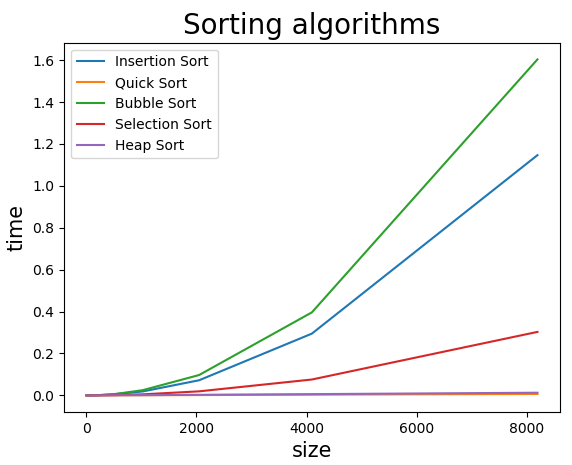
\includegraphics[width=0.6\textwidth]{../plots/sorting_plot.png}  
		\caption{Benchmark of all the implemented sorting algorithms.}
		\label{sortings}
	\end{figure}
	\noindent In Figure \ref{heap_quick} we compare the two best algorithms, \texttt{HEAP SORT} and \texttt{QUICKSORT}, by considering a wider range of input sizes. 
	
	\begin{figure}[h]
		\centering
		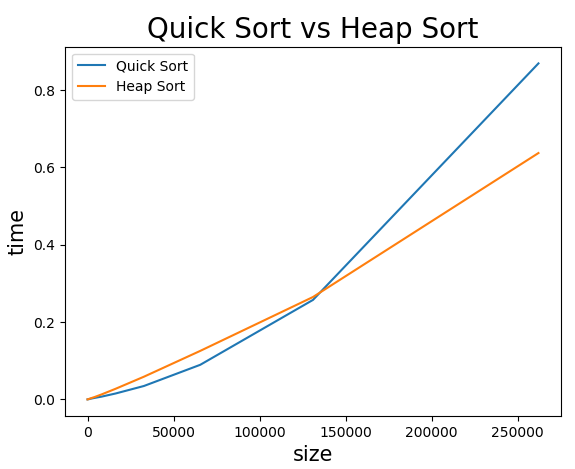
\includegraphics[width=0.6\textwidth]{../plots/quick_heap_sort_plot.png}  
		\caption{Benchmark of \texttt{HEAP SORT} and \texttt{QUICKSORT} with an input size that reaches $n=2^{18}$.}
		\label{heap_quick}
	\end{figure}
	\noindent It can be observed that starting from a size $n\simeq 1.5 \cdot 10^5$ \texttt{HEAP SORT} becomes faster than \texttt{QUICK SORT}.\\
	Figure \ref{quick_sort} and \ref{insertion_sort} report respectively the behaviour of \texttt{QUICK SORT} and \texttt{INSERTION SORT} for different scenarios.
	
	\newpage
	\begin{figure}[h]
		\hspace*{-3cm} 
		\begin{minipage}{.75\textwidth}
			\centering
			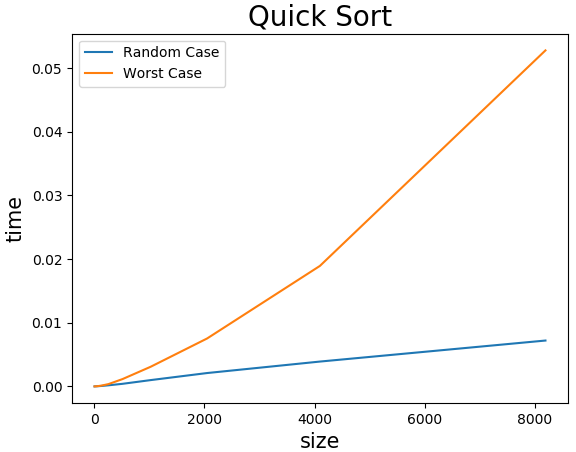
\includegraphics[width=.7\linewidth]{../plots/quick_sort_plot.png}
			\captionof{figure}{Benchmark of \texttt{INSERTION SORT} }
			\label{quick_sort}
		\end{minipage}%
	    \hspace*{-1.5cm} 
		\begin{minipage}{.75\textwidth}
			\centering
			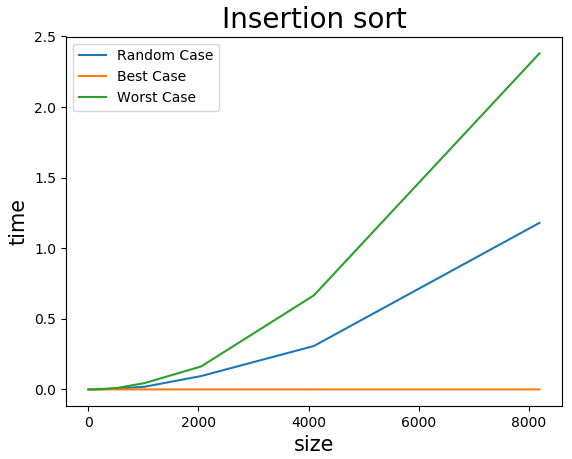
\includegraphics[width=.7\linewidth]{../plots/insertion_sort_plot.png}
			\captionof{figure}{Benchmark of \texttt{INSERTION SORT}.}
			\label{insertion_sort}
		\end{minipage}
	\end{figure}
	\noindent The curves show what expected from the theoretical results. Figure \ref{quick_sort} shows that for \texttt{QUICK SORT} the worst-case looks to have a quadratic behaviour, while the random-case is more fast, confirming a complexity that is $\Theta(n\log n)$. Figure \ref{insertion_sort} shows the result for \texttt{INSERTION SORT}; confirming the observation made before in Figure \ref{sortings}, the random case seems to be closer to the worst-case behaviour, which shows a quadratic shape, rather than the best-case that results to increase linearly.

	\section*{Exercise 3}
	\textbf{Argue about the following statement and answer the questions:}
	\begin{enumerate}[label=(\alph*)]
		\item \textbf{\texttt{HEAP SORT} on a array $A$ whose length is $n$ takes time} $O(n)$. 
		Since \texttt{HEAP SORT} complexity is given by the complexity of one single call of \texttt{BUILD HEAP} (which is $\Theta(n)$) and $n$ calls of \texttt{EXTRACT MIN} (which is $O(\log i)$, where $i$ is relative number of nodes in the heap) the overall cost of \texttt{HEAP SORT} is $O(n\log n)$. This higher bound represent a greater one respect to $O(n)$; thus in general \texttt{HEAP SORT} on a array $A$ of length $n$ doesn't take time $O(n)$. \\
		However, in a specific case in which the heap is built in such a way that \texttt{EXTRACT MIN} costs $\Theta(1)$, then the overall cost is $\Theta(n)$ and the statement holds.
		
		 
		\item \textbf{\texttt{HEAP SORT} on a array $A$ whose length is $n$ takes time} $\Omega(n)$. 
		As we explained in the point (a), we know that \texttt{HEAP SORT} in the best-case scenario has an overall cost of $\Theta(n)$. Then, since $T_{HS} (n) = \Theta(n)$ this is equivalent to say that  $T_{HS} (n) = \Omega(n)$ and, at the same time, $T_{HS} (n) = O(n)$. Thus, if this lower bound holds for the best scenario will also hold for every possible case and we conclude that the statement is true. 
		
		\item \textbf{What is the worst case complexity for \texttt{HEAP SORT}?}\\
		The worst-case scenario in \texttt{HEAP SORT} is that one in which we do $n$ calls of \texttt{EXTRACT MIN} operation and for every iteration $i$ the cost of this function is $\Theta(\log i)$, where $i$ is the relatives number of nodes down the heap. Thus,
		\begin{equation*}
		T_{HS} (n) = \Theta(n) + \sum_{i=1}^{n} \Theta(\log i) = \Theta(n) + \Theta(n\log n) = \Theta(n\log n).  
		\end{equation*}
		
		\item \textbf{\texttt{QUICK SORT} on a array $A$ whose length is $n$ takes time} $O(n^3)$. 
		On an array $A$ of length $n$ \texttt{QUICK SORT} has on average a time performance $T_{QS} = \Theta(n \log_2 n) $.  This will mean that on average $T_{QS}$ is both $O(n\log_2 n)$ and $\Omega(n\log_2 n)$. Since $O(n\log_2 n) \subset O(n^3)$ we can say that on  average \texttt{QUICK SORT} takes time $O(n^3)$. However, using such higher bound it cannot be useful during performance analysis since we have found, in this case $n\log_2 n$, a cheaper function that can be a bound to our complexity function. 
		The same reasoning can be applied to the worst-case scenario which has complexity equal to $\Theta(n^2) $.
		
		\item \textbf{What is the complexity of \texttt{QUICK SORT}?}\\
		As already stated in the previous point the complexity of \texttt{QUICK SORT} is on average and in the optimal case $\Theta(n\log n)$, while for the worst-case is $\Theta(n^2)$.
		\item \textbf{\texttt{BUBBLE SORT} on a array $A$ whose length is $n$ takes time} $\Omega(n)$.
		Since \texttt{BUBBLE SORT} involves two loops over the length $n$ of the array $A$, for any scenario the complexity of \texttt{BUBBLE SORT} is $\Theta(n^2)$. Automatically, \texttt{BUBBLE SORT} takes time $\Omega(n^2)$ and because $\Omega(n^2) \subset \Omega(n) $ we can conclude that the statement is formally true. However, we know that there exists a lower bound, in this case $n^2$, higher than $n$ and so this sentence is not useful in a performance analysis. 
		\item  \textbf{What is the complexity of \texttt{BUBBLE SORT}?} \\
		As said before,  \texttt{BUBBLE SORT} involves two loops over the length $n$ of the array $A$, then for any scenario the complexity of \texttt{BUBBLE SORT} is $\Theta(n^2)$. 
	\end{enumerate}

	\section*{Exercise 4}
	\textbf{Solve the following recursive equation:}
	$$
	T(n) = \begin{cases}
			\Theta(1) & \text{if } n= 32 \\
			3T(\frac{n}{4}) + \Theta(n^{3/2}) & \text{otherwise}
			\end{cases} 
	$$
	
	\noindent Let's use the above the relation in order to build a recursion tree.  each node represents the cost of a single sub-problem somewhere in the set of recursive function invocations. We sum the costs within each level of the tree to obtain a set of per-level costs, and then we sum all the per-level costs to determine the total cost of all levels of the recursion. For convenience, we assume that $n$ is an exact power of $4$, so that all sub-problem sizes are integers. \\
	
	
	\begin{figure}[h]

	\begin{center}
		
	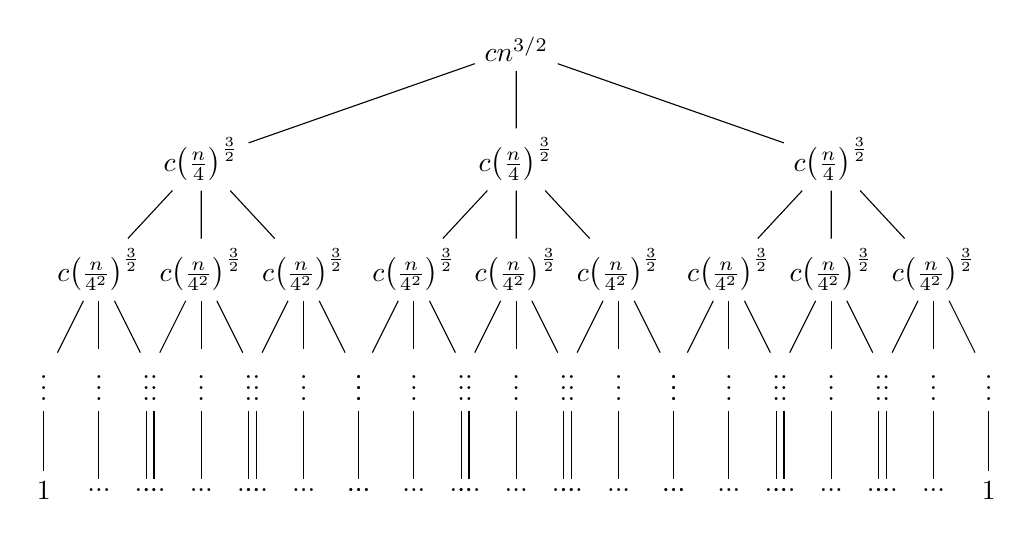
\begin{tikzpicture}[level distance=1.4cm,
	level 1/.style={sibling distance=4cm},
	level 2/.style={sibling distance=1.3cm},
	level 3/.style={sibling distance=0.7cm},
	level 4/.style={sibling distance=0.4cm},
	level 5/.style={sibling distance=0.2cm}]
	\node {$cn^{3/2}$}
	child {node {$c\big(\frac{n}{4}\big)^{\frac{3}{2}}$}
		child {node {$c\big(\frac{n}{4^2}\big)^{\frac{3}{2}}$}
			    child {
			    	node {$\vdots$}
		     	        child {node {$1$} 
		     	        }
	     	         }
	     	     child {
	     	     	    node {$\vdots$}
     	     	    	child {node{$...$} 
          	    	    }
              	      }  
     	     	 child {
     	     	 	node {$\vdots$}
     	     	 	child {node{$...$} 
     	     	 	}
     	     	 }  
          }
	     child {node {$c\big(\frac{n}{4^2}\big)^{\frac{3}{2}}$}
	     	child {
	     		node {$\vdots$}
	     		child {node {$...$} 
	     		}
	     	}
	     	child {
	     		node {$\vdots$}
	     		child {node{$...$} 
	     		}
	     	}  
	     	child {
	     		node {$\vdots$}
	     		child {node{$...$} 
	     		}
	     	}  
	     }
		child {node {$c\big(\frac{n}{4^2}\big)^{\frac{3}{2}}$}
			child {
				node {$\vdots$}
				child {node {$...$} 
				}
			}
			child {
				node {$\vdots$}
				child {node{$...$} 
				}
			}  
			child {
				node {$\vdots$}
				child {node{$...$} 
				}
			}  
		}
	}
	child {node {$c\big(\frac{n}{4}\big)^{\frac{3}{2}}$}
		child {node {$c\big(\frac{n}{4^2}\big)^{\frac{3}{2}}$}
			child {
				node {$\vdots$}
				child {node {$...$} 
				}
			}
			child {
				node {$\vdots$}
				child {node{$...$} 
				}
			}  
			child {
				node {$\vdots$}
				child {node{$...$} 
				}
			}  
		}
		child {node {$c\big(\frac{n}{4^2}\big)^{\frac{3}{2}}$}
			child {
				node {$\vdots$}
				child {node {$...$} 
				}
			}
			child {
				node {$\vdots$}
				child {node{$...$} 
				}
			}  
			child {
				node {$\vdots$}
				child {node{$...$} 
				}
			}  
		}
		child {node {$c\big(\frac{n}{4^2}\big)^{\frac{3}{2}}$}
			child {
				node {$\vdots$}
				child {node {$...$} 
				}
			}
			child {
				node {$\vdots$}
				child {node{$...$} 
				}
			}  
			child {
				node {$\vdots$}
				child {node{$...$} 
				}
			}  
		}
	}
	child {node {$c\big(\frac{n}{4}\big)^{\frac{3}{2}}$}
		child {node {$c\big(\frac{n}{4^2}\big)^{\frac{3}{2}}$}
			child {
				node {$\vdots$}
				child {node {$...$} 
				}
			}
			child {
				node {$\vdots$}
				child {node{$...$} 
				}
			}  
			child {
				node {$\vdots$}
				child {node{$...$} 
				}
			}  
		}
		child {node {$c\big(\frac{n}{4^2}\big)^{\frac{3}{2}}$}
			child {
				node {$\vdots$}
				child {node {$...$} 
				}
			}
			child {
				node {$\vdots$}
				child {node{$...$} 
				}
			}  
			child {
				node {$\vdots$}
				child {node{$...$} 
				}
			}  
		}
		child {node {$c\big(\frac{n}{4^2}\big)^{\frac{3}{2}}$}
			child {
				node {$\vdots$}
				child {node {$...$} 
				}
			}
			child {
				node {$\vdots$}
				child {node{$...$} 
				}
			}  
			child {
				node {$\vdots$}
				child {node{$1$} 
				}
			}  
		}
	};
	\end{tikzpicture}
	\caption{Recursion tree} \label{recursion_tree}
	\end{center}
	
	\end{figure}
	
	\noindent Given the tree at Figure \ref{recursion_tree}, I add up the costs over all levels to determine the cost for the entire tree:
	\begin{eqnarray}
	\nonumber
	T(n) &=& cn^{3/2} + \frac{3}{4^{3/2}} cn^{3/2} + ... + \Bigg( \frac{3}{4^{3/2}} \Bigg)^{\log_4 (n/32)-1} cn^{3/2} + \Theta(n^{\log_4 3}),\\
	\nonumber
	&=& cn^{3/2} + \frac{3}{8} cn^{3/2} + ... + \Bigg( \frac{3}{8} \Bigg)^{\log_4 (n/32)-1} cn^{3/2} + \Theta(n^{\log_4 3}), \\ 
	\nonumber
	&=& cn^{3/2} \sum_{i=0}^{\log_4 (n/32)-1} \Bigg( \frac{3}{8} \Bigg)^i + \Theta(n^{\log_4 3}), 
	\nonumber
	\end{eqnarray}
	
	\begin{eqnarray}
	\nonumber
	&=& cn^{3/2} \sum_{i=0}^{\log_4 (n/32)-1} \Bigg( \frac{3}{8} \Bigg)^i + \Theta(n^{\log_4 3}), \\
	\nonumber
	&\leq &   cn^{3/2} \sum_{i=0}^{+\infty} \Bigg( \frac{3}{8} \Bigg)^i + \Theta(n^{\log_4 3}), \\
	\nonumber
	 & = &   \frac{8}{5} cn^{3/2} + \Theta(n^{\log_4 3}) ~ ~ \in O(n^{3/2}) .
	\end{eqnarray}
	
	Thus, $ T(n) \in O(n^{3/2}) $. 
	
\end{document}